\subsection{Prototipo mínimo viable}
El proyecto tiene como finalidad desarrollar una pagina web que ofrezca recomendaciones confiables y enfocados en la seguridad y comodidad de los nómadas digitales que se encuentran en Bogotá. El desarrollo se llevará a cabo usando arquitecturas y herramientoas que den pie a la creación de
una plataforma sostenible, escalable y dispuesta a las necesidades de los usuarios, primando la experiencia del usuario a traves de la seguridad y confianza en la información que se le brinda.

\textbf{Tecnologías}
\begin{itemize}
    \item \textbf{Spring Boot: } Spring Boot es un framework de desarrollo de aplicaciones Java que simplifica la creación de aplicaciones empresariales. Proporciona una configuración automática y una amplia gama de herramientas para facilitar el desarrollo, lo que permite a los desarrolladores centrarse en la lógica del negocio en lugar de la configuración del entorno.
    Spring Boot es especialmente útil para crear aplicaciones web y servicios RESTful, ya que incluye características como la gestión de dependencias, la configuración de seguridad y la integración con bases de datos. Además, permite el despliegue rápido de aplicaciones en entornos de producción, lo que lo convierte en una opción popular para el desarrollo ágil.
    \vspace{2mm}
    \begin{minipage}{0.9\textwidth}
        \centering
        \captionof{figure}[{Logo Spring Boot}]{ Logo Spring Boot  }
        \label{Firestore}
         
\includegraphics[width=0.3\textwidth]{Content/Images/spring-boot-logo.png}
        \footnote{Nota. \textup{Fuente: spring.io}}
    \end{minipage}

    \item \textbf{Angular: } Angular es un framework web que permite a los desarrolladores crear aplicaciones rápidas y fiables.
    Mantenido por un equipo dedicado de Google, Angular ofrece un amplio conjunto de herramientas, API y bibliotecas para simplificar y optimizar tu flujo de trabajo de desarrollo. Angular te ofrece una plataforma sólida para crear aplicaciones rápidas y fiables que escalan con el tamaño de tu equipo y de tu código fuente.

    Angular es muy util para el desarrollo de aplicaciones web modernas, ya que permite crear interfaces de usuario dinámicas y reactivas. Su enfoque basado en componentes facilita la reutilización del código y mejora la mantenibilidad de las aplicaciones. Además, Angular cuenta con un ecosistema robusto que incluye herramientas para pruebas, enrutamiento y gestión del estado, lo que lo convierte en una opción popular para el desarrollo de aplicaciones empresariales.
    
    \vspace{2mm}
    \begin{minipage}{0.9\textwidth}
        \centering
        \captionof{figure}[{Logo Angular}]{Logo Angular}
        \label{angularLogo}
        
\includegraphics[width=0.25\textwidth]{Content/Images/angular-logo.png}
        \footnote{Nota. \textup{Fuente: angular.io}}
    \end{minipage}
    
    \item \textbf{PostgreSQL: } PostgreSQL es un potente sistema de base de datos relacional de objetos de código abierto con más de 35 años de desarrollo activo eso le ha valido una sólida reputación de confiabilidad, robustez de características y rendimiento.

    La comunidad de código abierto proporciona muchos lugares útiles para familiarizarse con PostgreSQL, incluyendo la documentación oficial, tutoriales y foros de discusión. PostgreSQL es conocido por su capacidad para manejar grandes volúmenes de datos y transacciones complejas, lo que lo convierte en una opción popular para aplicaciones empresariales y sistemas de gestión de datos críticos.
    \vspace{2mm}
    \begin{minipage}{0.9\textwidth}
        \centering
        \captionof{figure}[{Logo PostgreSQL}]{Logo PostgreSQL}
        \label{postgresqlLogo}
        
\includegraphics[width=0.3\textwidth]{Content/Images/postgresql-logo.png}
        \footnote{Nota. \textup{Fuente: postgresql.org}}
    \end{minipage}
    \item \textbf{Inteligencias artificiales:}En el desarrollo de este proyecto, se contempló la integración de diversas inteligencias artificiales para mejorar la experiencia del usuario y optimizar el rendimiento de la plataforma. Estas IA se utilizarán para analizar datos, personalizar recomendaciones y mejorar la seguridad del sistema. Algunas de las aplicaciones específicas incluyen:
        \begin{itemize}
            \item \textbf{Análisis de datos: } Utilizar IA para procesar y analizar grandes volúmenes de datos, identificando patrones y tendencias que pueden ser útiles para los usuarios,para esto se emplean NPL (Natural Language Processing) para el análisis de reseñas y comentarios de los usuarios, permitiendo una comprensión más profunda de las necesidades y preferencias de los nómadas digitales.
            \item \textbf{Recomendaciones personalizadas: } Implementar embeddings los cuales permiten capturar relaciones semánticas y contextuales entre palabras para ofrecer recomendaciones personalizadas basadas en las preferencias y comportamientos de los usuarios, mejorando la relevancia de las sugerencias de lugares y servicios, además de que permite recomendaciones explicables y fundamentadas.
            \item \textbf{Seguridad: } Emplear IA para detectar y prevenir amenazas de seguridad, mejorando la protección de los datos sensibles de los usuarios además de la detección de fraudes y actividades sospechosas en la plataforma, este haciendo analisis de datos de usuarios sospechosos.

\end{itemize}

\vspace{5mm}
\textbf{Arquitectura} 

\begin{itemize}
    \item\textbf{Arquitectura de microservicios: }Los microservicios son una arquitectura de software donde la aplicación se divide en pequeños servicios independientes, cada uno con una función específica (ej.: autenticación, procesamiento de pagos, geolocalización), que se comunican entre sí mediante APIs. A diferencia de las aplicaciones monolíticas, cada microservicio puede desarrollarse, desplegarse y escalarse por separado, usando tecnologías distintas según su necesidad.
        Esta arquitectura permite escalar selectivamente funciones críticas (como alertas en tiempo real o validación de zonas), integrar tecnologías diversas y aislar fallos sin colapsar todo el sistema. Además, facilita la expansión modular a nuevas ciudades y optimiza costos en la nube al escalar solo lo necesario
        \vspace{2mm}
        \begin{center}
        \begin{minipage}{0.9\textwidth}
            \centering
            \captionof{figure}[{Arquitectura de Microservicios.}]{Ejemplo de arquitectura de microservicios.}
            \label{microservicios}
            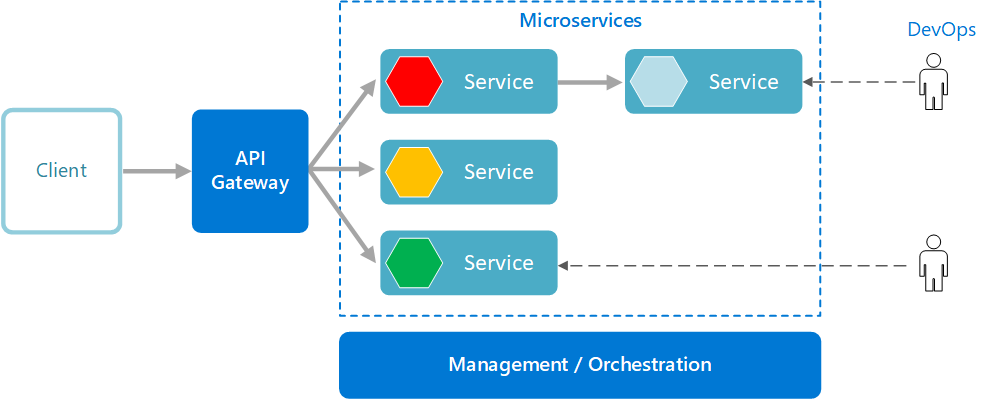
\includegraphics[width=0.9\textwidth]{Content/Images/microservices-logical.png}
            \footnote{Nota. \textup{Fuente: learn.microsoft.com/es-es/azure/architecture/guide/architecture-styles/microservices}}
        \end{minipage}
        \end{center}
        \item \textbf{Arquitectura hexagonal: } La arquitectura hexagonal, también llamada arquitectura de puertos y adaptadores, es un enfoque propuesto por Alistair Cockburn que estructura el software en capas para separar claramente las funcionalidades. Su objetivo principal es mantener el núcleo del sistema (el dominio) aislado, permitiendo que las interacciones con servicios externos (como bases de datos o APIs) se realicen a través de adaptadores específicos.

Gracias a esta separación, los distintos componentes del sistema pueden evolucionar y mantenerse de forma independiente, lo que facilita tanto la escalabilidad como la integración de nuevas tecnologías o servicios. En este modelo, el dominio central permanece protegido de los cambios externos, mientras que los adaptadores gestionan la comunicación con el entorno.
Al hacer uso de esta arquitectura, se tienen diversos beneficios y ventajas con respecto a otras arquitecturas, como los despliegues independientes donde cada componente tales como análisis de reseñas,monitorización de alertas, validación de zonas entre otros, pueden ser desplegados, ser actualizados o revertir cambios sin necesidad de poner offline toda la aplicación. 
Se tiene la facilidad de poder escalar cada componente de forma independiente, lo que permite que la aplicación pueda crecer y adaptarse componente por componente, optimizando costos y recursos.Tambien se tiene la capacidad de cumplir con estandares de manejo de datos sensibles como cifrado reforzado sin complicar el resto de la plataforma. Además , se facilita la integración de nuevas tecnologías o servicios, ya que los adaptadores permiten conectar el núcleo del sistema con diferentes fuentes de datos o APIs sin afectar la lógica central.

    \vspace{2mm}
    \begin{minipage}{0.9\textwidth}
        \centering
        \captionof{figure}[{Arquitectura Hexagonal.}]{Ejemplo de arquitectura hexagonal.}
        \label{hexagonal}
        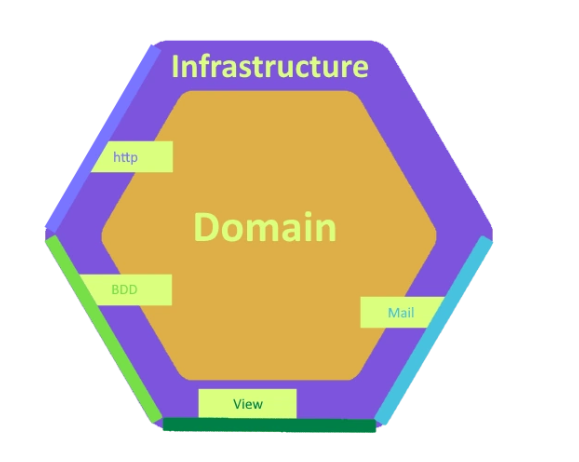
\includegraphics[width=0.9\textwidth]{Content/Images/hexagonal.png}
        \footnote{Nota. \textup{Fuente: https://softwarecrafters.io/react/arquitectura-hexagonal-frontend}}
    \end{minipage}
\vspace{2mm}
\begin{minipage}{0.9\textwidth}
    \centering
    \captionof{figure}[{Arquitectura Hexagonal.}]{Ejemplo de arquitectura hexagonal.}
    \label{hexagonal}
    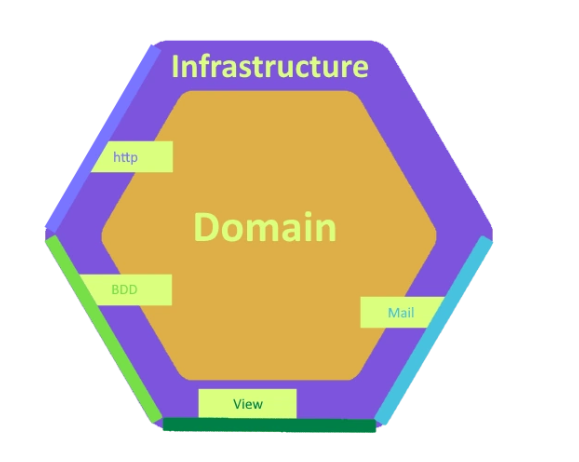
\includegraphics[width=0.5\textwidth]{Content/Images/hexagonal.png}
    \footnote{Nota. \textup{Fuente: https://softwarecrafters.io/react/arquitectura-hexagonal-frontend}}
\end{minipage}
    
\end{itemize}
\textbf{Infraestructura}
\newline
La computación en la nube constituye un pilar esencial para este proyecto, ya que posibilita el acceso y la provisión de almacenamiento, servidores, aplicaciones y otros recursos a través de Internet bajo un modelo de pago por uso. En vez de depender de infraestructuras físicas o centros de datos locales, se recurre a servicios remotos y gestionados, lo que facilita la escalabilidad y optimiza la administración de los recursos.

En este contexto, se ha optado por AWS Lightsail como plataforma en la nube. AWS Lightsail proporciona una infraestructura sencilla y rentable que facilita tanto el desarrollo como el despliegue de aplicaciones, ofreciendo servicios como servidores virtuales, almacenamiento, bases de datos y gestión de redes, todo desde una única plataforma. Esto elimina la necesidad de gestionar servidores físicos o realizar configuraciones complejas, permitiendo que el equipo de desarrollo se concentre en la creación de la aplicación. 
\newline
\textbf{Software as a Service (SaaS):}
El modelo SaaS (Software como Servicio) es ampliamente utilizado en este proyecto, ya que AWS Lightsail permite implementar soluciones bajo este enfoque. Al tratarse de un servicio gestionado, Lightsail permite a los desarrolladores enfocarse en el desarrollo del software sin preocuparse por la administración de servidores físicos, actualizaciones de seguridad o gestión de licencias. Los usuarios pueden acceder a la aplicación y sus funcionalidades desde cualquier lugar con conexión a Internet, lo que simplifica tanto el uso como la operación del sistema. 

\textbf{Requisitos}

\begin{enumerate}
    \item Funcionales
        \par\vspace{2mm}
        \begin{minipage}{0.9\textwidth}
        \centering
        \captionof{table}[{Requisitos funcionales.}]{ Requisitos funcionales.}
        \label{req1}
        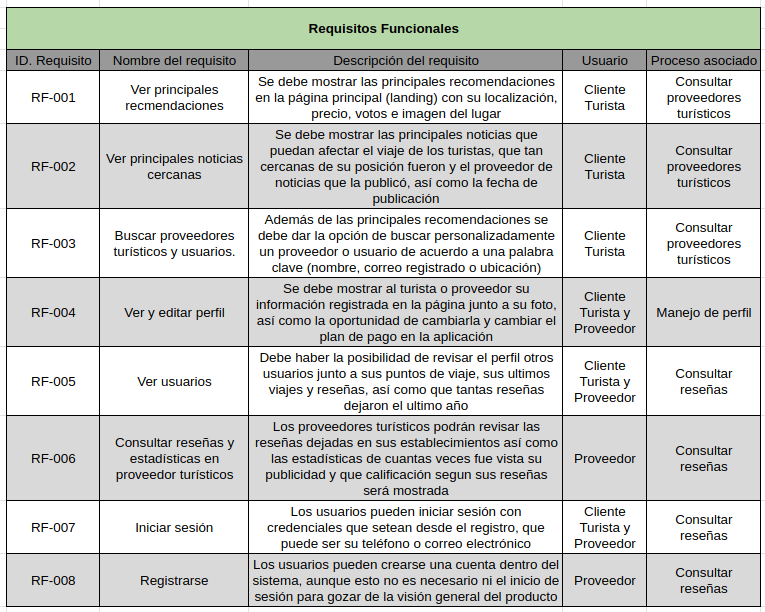
\includegraphics[width=1\textwidth]{Content/Images/requisitos.png}
        \footnote{}{Nota. \textup{Fuente : Autores.}}
        \end{minipage}
           
    \item No funcionales
    \par\vspace{2mm}
        \begin{minipage}{0.9\textwidth}
        \centering
        \captionof{table}[{Requisitos no funcionales.}]{ Requisitos no funcionales.}
        \label{req1}
        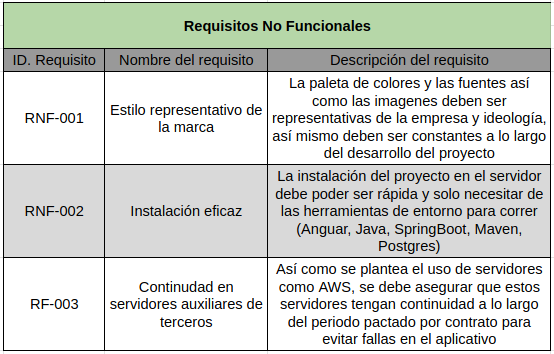
\includegraphics[width=1\textwidth]{Content/Images/requisitosNF.png}
        \footnote{}{Nota. \textup{Fuente : Autores.}}
        \end{minipage}
        
\end{enumerate}

\textbf{Casos de uso}

    \vspace{2mm}
    \begin{minipage}{0.9\textwidth}
    \centering
    \captionof{figure}[{Diagramas de caso de uso.}]{Diagramas de caso de uso.}
    \label{caso1}
    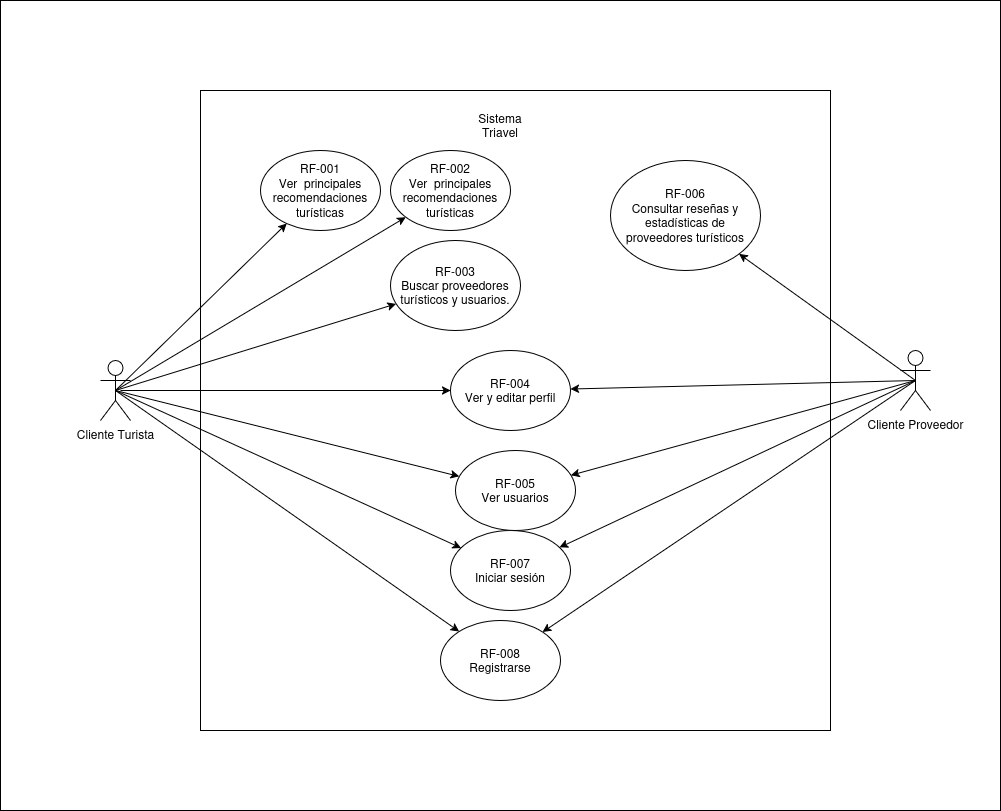
\includegraphics[width=0.9\textwidth]{Content/Images/CasosDeUso.png}
    \footnote{Nota. \textup{Fuente : Autores.}}
    \end{minipage}
    %------------------------------------------------------------------%


\textbf{Vistas principales del prototipo}
En función de los requisitos funcionales, no funcionales y los casos de uso definidos, a continuación se presentan en las figuras \ref{prot1}, \ref{prot2}, \ref{prot3}, \ref{prot4}, \ref{prot5}, \ref{prot6}, \ref{prot7}, \ref{prot8} , \ref{prot9} , \ref{prot10} ,\ref{prot11} ,\ref{prot12} las principales vistas que conforman el núcleo del plan de negocio. Todas las imágenes mostradas en este prototipo fueron diseñadas y desarrolladas exclusivamente para este proyecto.

    \vspace{2mm}
    \begin{minipage}{0.9\textwidth}
    \centering
    \captionof{figure}[{Vista principal parte I}]{ Vista principal parte I}
    \label{prot1}
    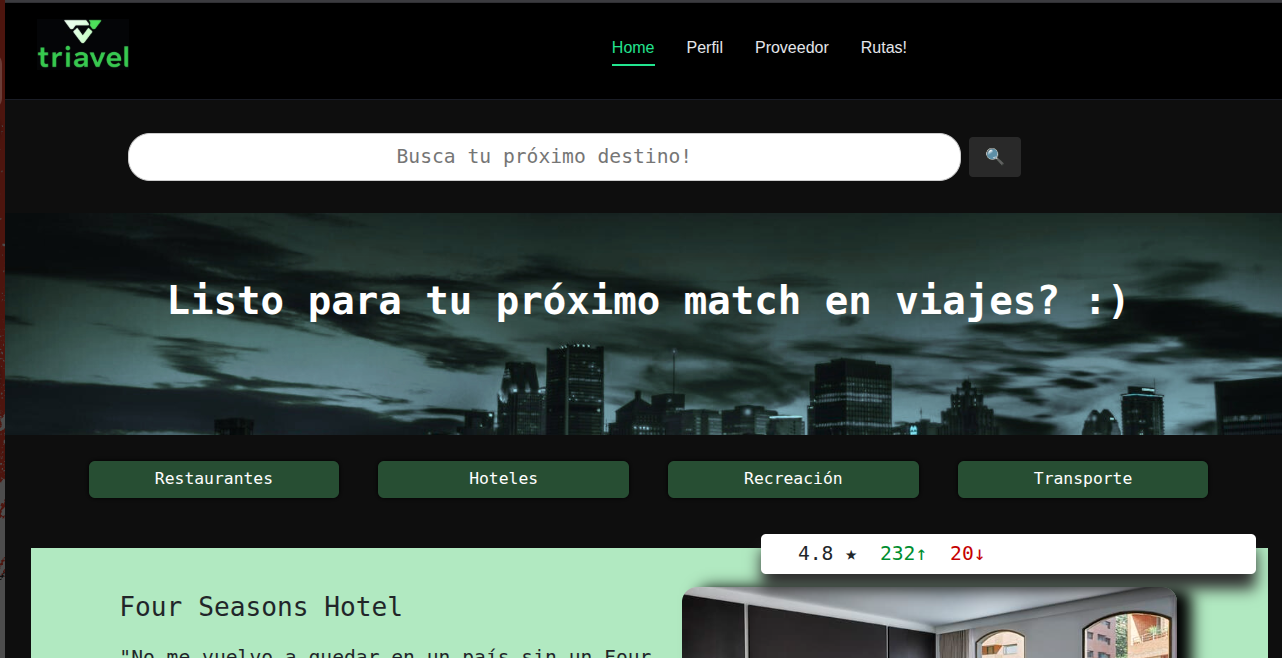
\includegraphics[width=0.9\textwidth]{Content/Images/VistaGeneral1.png}
    \footnote{Nota. \textup{Fuente: Autores}}
    \end{minipage}

    \vspace{2mm}
    \begin{minipage}{0.9\textwidth}
    \centering
    \captionof{figure}[{Vista principal parte II}]{ Vista principal parte II}
    \label{prot2}
    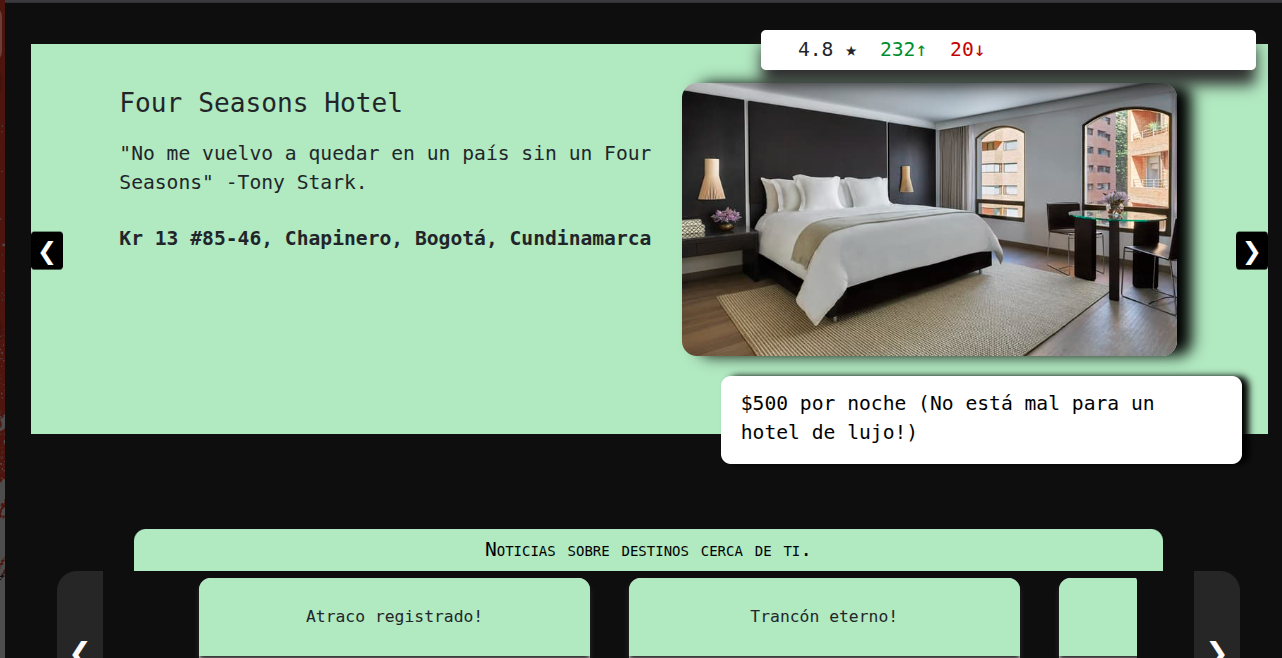
\includegraphics[width=0.9\textwidth]{Content/Images/VistaGeneral2.png}
    \footnote{Nota. \textup{Fuente: Autores}}
    \end{minipage}

    \vspace{2mm}
    \begin{minipage}{0.9\textwidth}
    \centering
    \captionof{figure}[{Vista principal parte III}]{ Vista principal parte III}
    \label{prot3}
    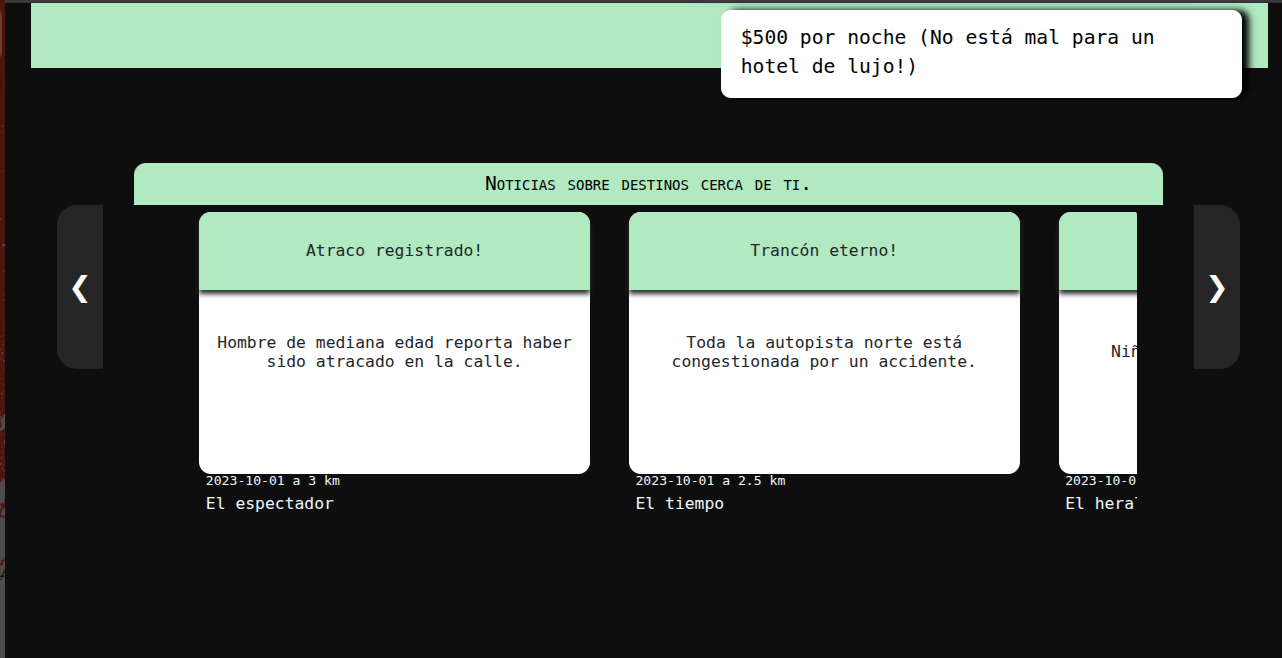
\includegraphics[width=0.9\textwidth]{Content/Images/VistaGeneral3.png}
    \footnote{Nota. \textup{Fuente: Autores}}
    \end{minipage}

    \vspace{2mm}
    \begin{minipage}{0.9\textwidth}
    \centering
    \captionof{figure}[{Tu Perfil}]{Tu Perfil}
    \label{prot4}
    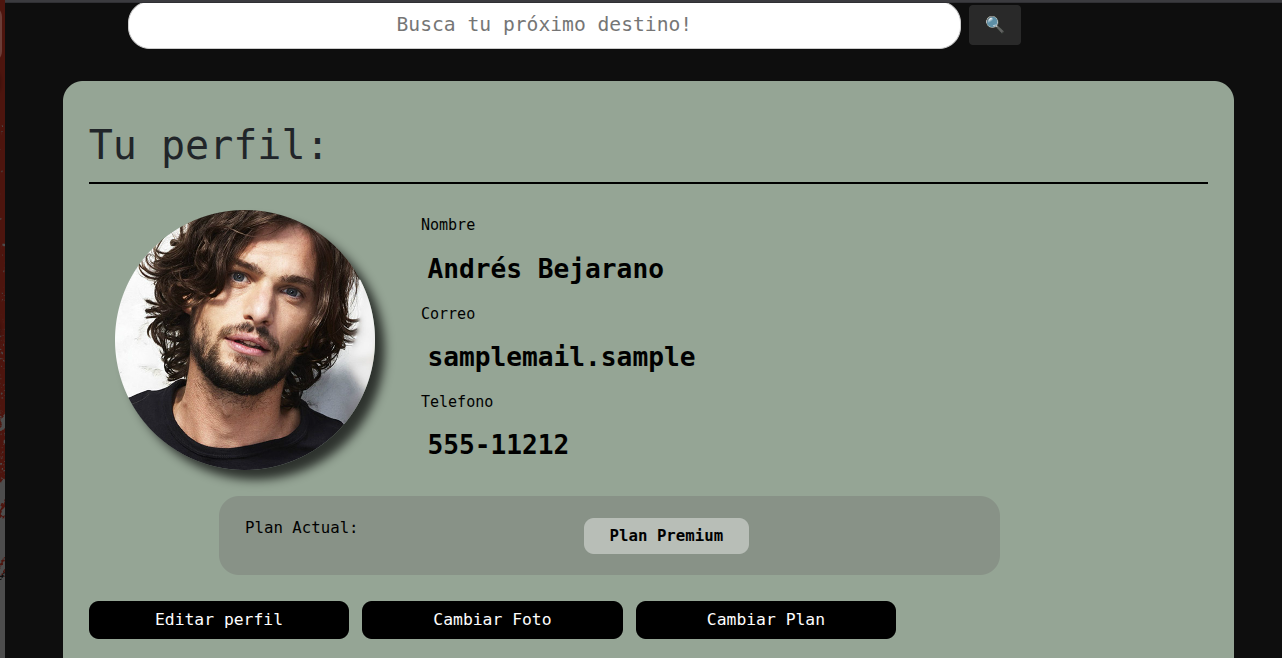
\includegraphics[width=0.9\textwidth]{Content/Images/TuPerfil.png}
    \footnote{Nota. \textup{Fuente: Autores}}
    \end{minipage}

     \vspace{2mm}
    \begin{minipage}{0.9\textwidth}
    \centering
    \captionof{figure}[{Vista de proveedor Parte I}]{Vista de proveedor Parte I}
    \label{prot5}
    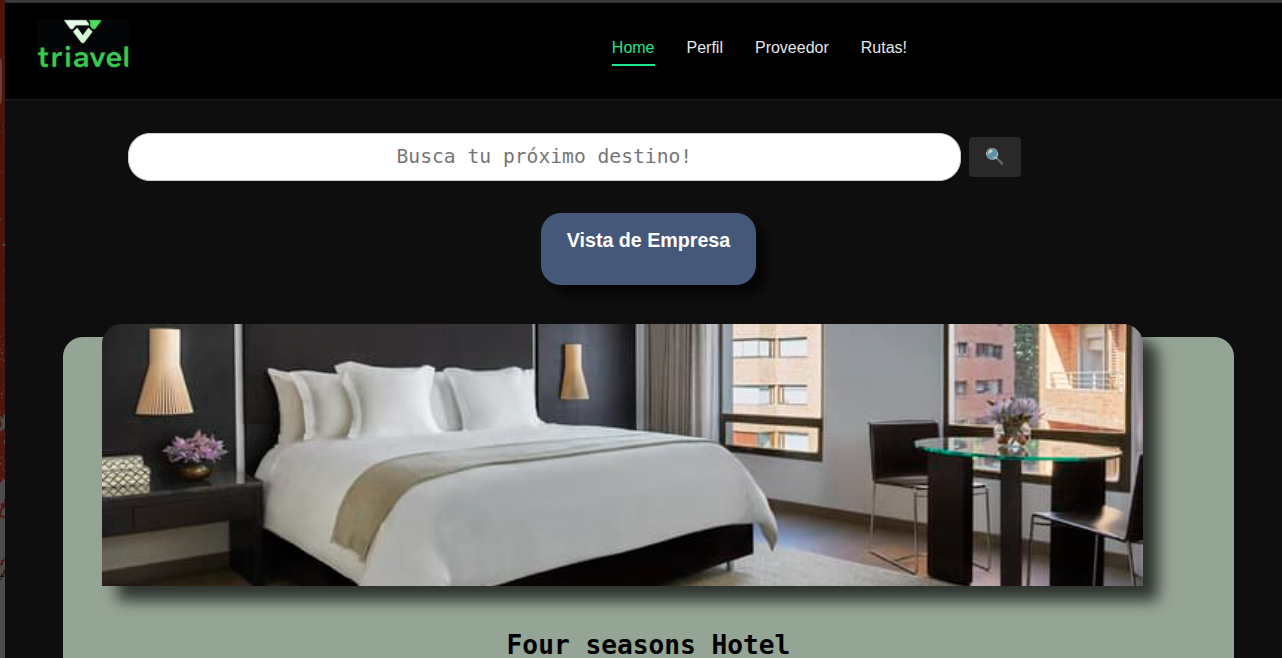
\includegraphics[width=0.9\textwidth]{Content/Images/VistaProveedor1.png}
    \footnote{Nota. \textup{Fuente: Autores}}
    \end{minipage}

     \vspace{2mm}
    \begin{minipage}{0.9\textwidth}
    \centering
    \captionof{figure}[{Vista de proveedor Parte II}]{Vista de proveedor Parte II}
    \label{prot6}
    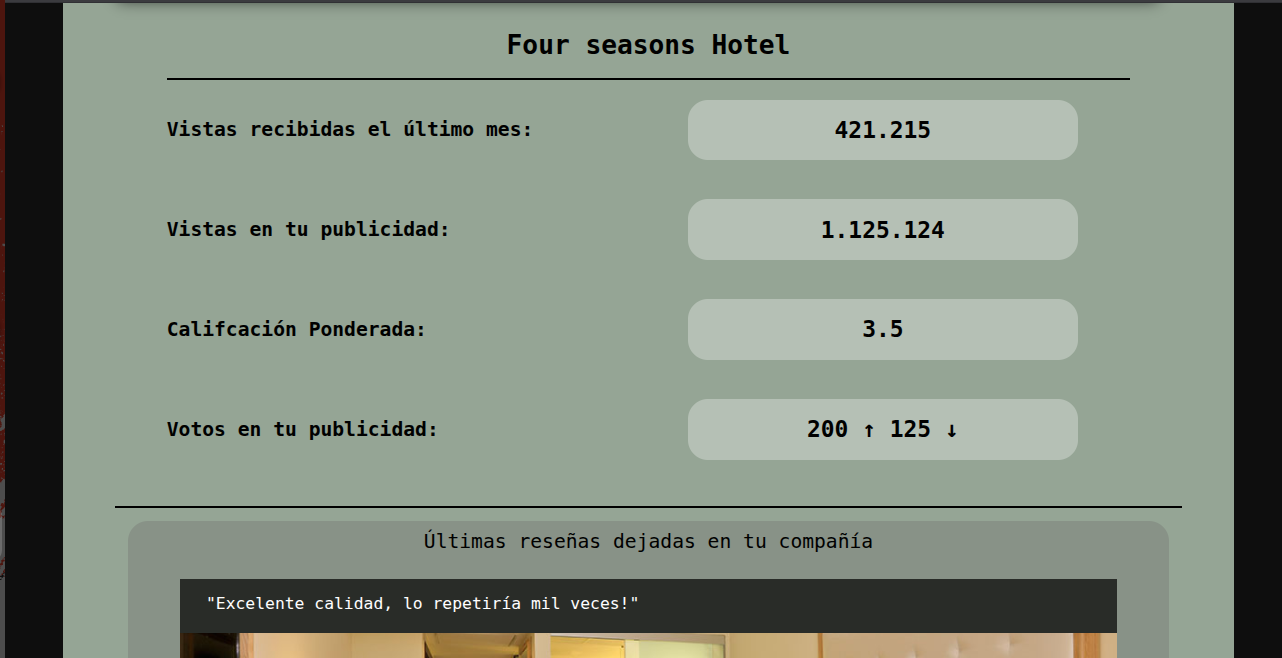
\includegraphics[width=0.9\textwidth]{Content/Images/VistaProveedor2.png}
    \footnote{Nota. \textup{Fuente: Autores}}
    \end{minipage}

     \vspace{2mm}
    \begin{minipage}{0.9\textwidth}
    \centering
    \captionof{figure}[{Vista de proveedor Parte III}]{Vista de proveedor Parte III}
    \label{prot7}
    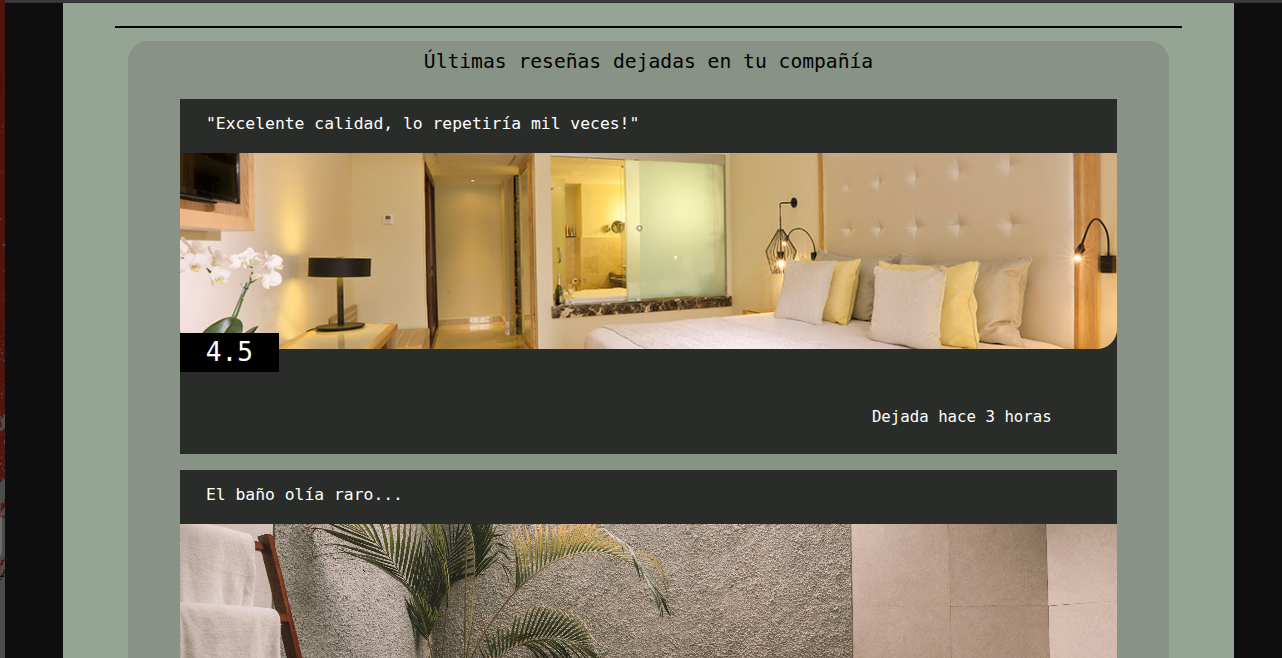
\includegraphics[width=0.9\textwidth]{Content/Images/VistaProveedor3.png}
    \footnote{Nota. \textup{Fuente: Autores}}
    \end{minipage}

     \vspace{2mm}
    \begin{minipage}{0.9\textwidth}
    \centering
    \captionof{figure}[{Ruta de viaje Parte I}]{Ruta de viaje Parte I}
    \label{prot8}
    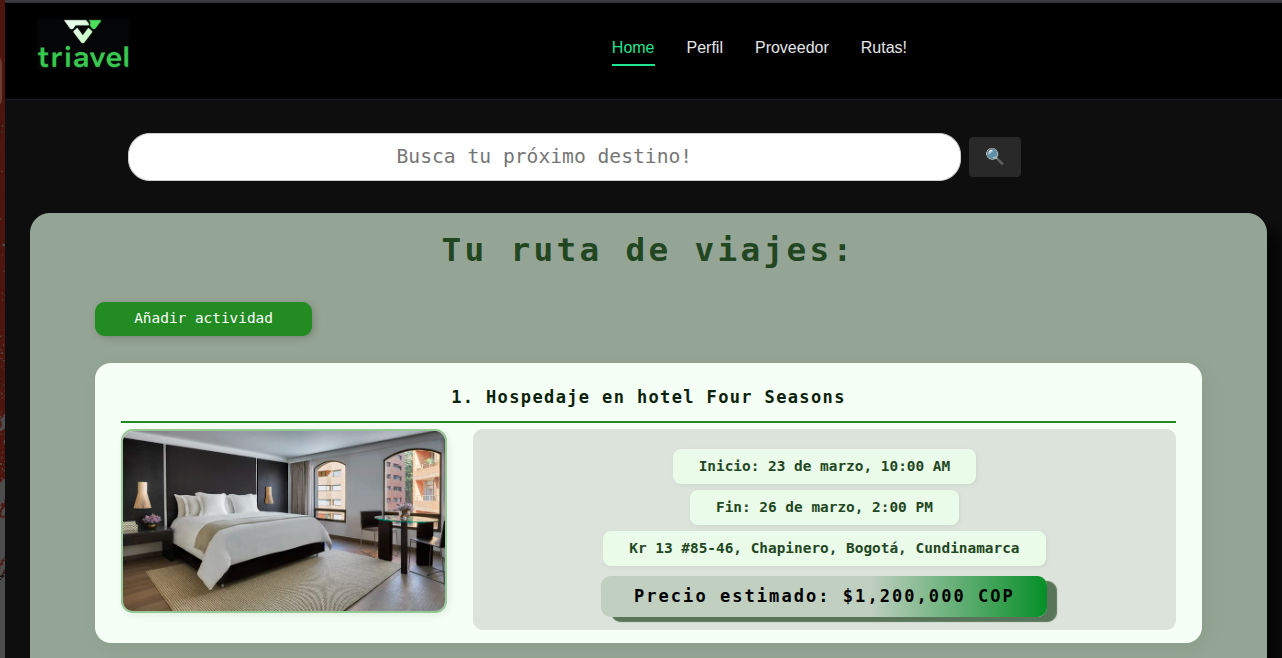
\includegraphics[width=0.9\textwidth]{Content/Images/RutaDeViaje1.png}
    \footnote{Nota. \textup{Fuente: Autores}}
    \end{minipage}

      \vspace{2mm}
    \begin{minipage}{0.9\textwidth}
    \centering
    \captionof{figure}[{Ruta de viaje Parte II}]{Ruta de viaje Parte II}
    \label{prot9}
    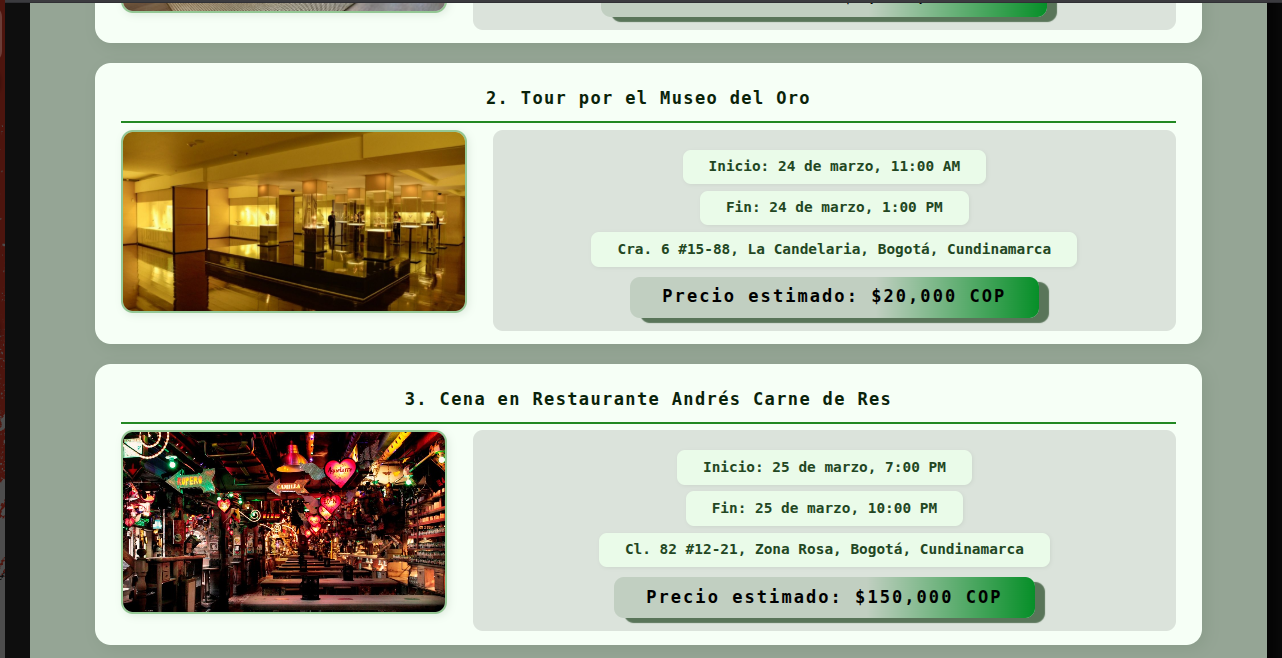
\includegraphics[width=0.9\textwidth]{Content/Images/RutaDeViaje2.png}
    \footnote{Nota. \textup{Fuente: Autores}}
    \end{minipage}

      \vspace{2mm}
    \begin{minipage}{0.9\textwidth}
    \centering
    \captionof{figure}[{Resultados de busqueda}]{Resultados de busqueda}
    \label{prot10}
    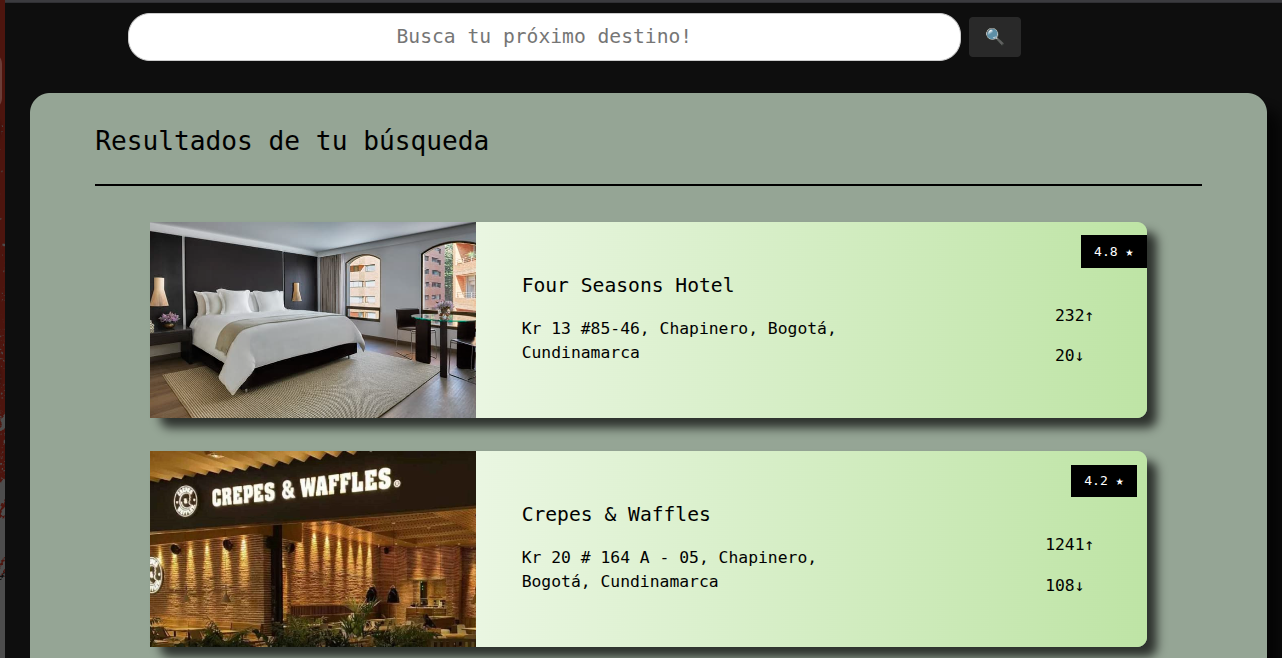
\includegraphics[width=0.9\textwidth]{Content/Images/ResultadosDeBusqueda.png}
    \footnote{Nota. \textup{Fuente: Autores}}
    \end{minipage}

       \vspace{2mm}
    \begin{minipage}{0.9\textwidth}
    \centering
    \captionof{figure}[{Vista de sitio}]{Vista de sitio}
    \label{prot11}
    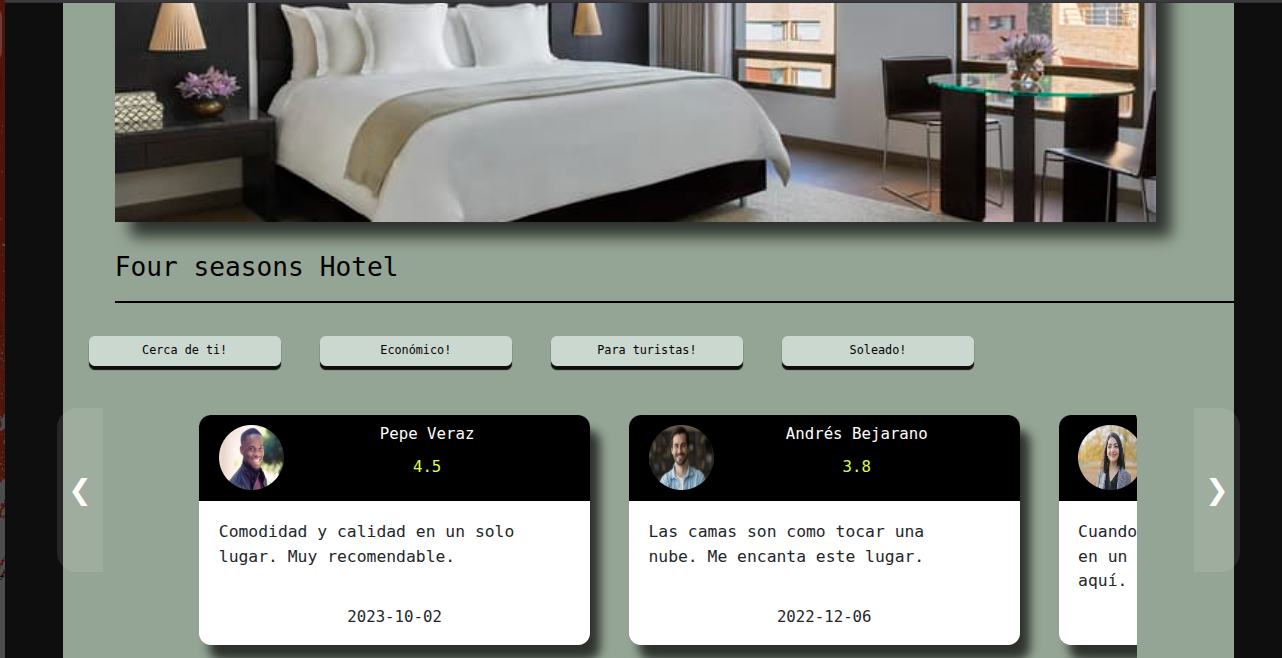
\includegraphics[width=0.9\textwidth]{Content/Images/VistaDeSitio.png}
    \footnote{Nota. \textup{Fuente: Autores}}
    \end{minipage}

      \vspace{2mm}
    \begin{minipage}{0.9\textwidth}
    \centering
    \captionof{figure}[{Perfil de usuario}]{Perfil de Usuario}
    \label{prot12}
    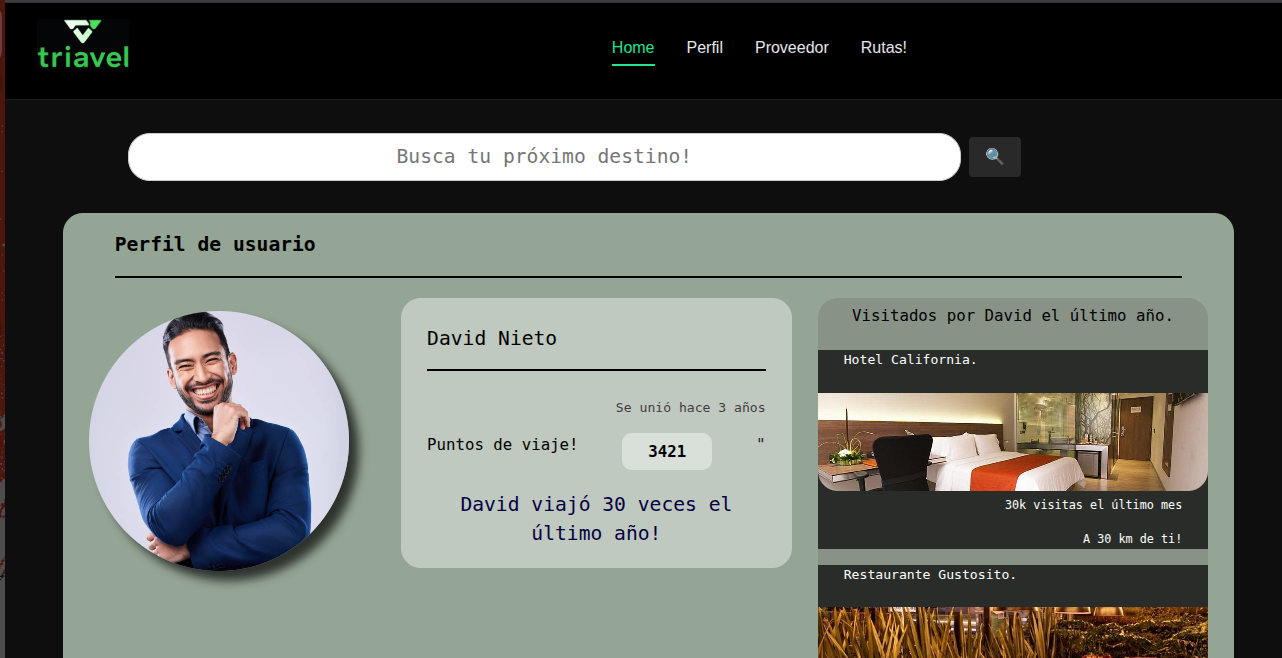
\includegraphics[width=0.9\textwidth]{Content/Images/UserProfile.png}
    \footnote{Nota. \textup{Fuente: Autores}}
    \end{minipage}

    

    
    